
% Default to the notebook output style

    


% Inherit from the specified cell style.




    
\documentclass{report}

    \usepackage{graphicx} % Used to insert images
    \usepackage{adjustbox} % Used to constrain images to a maximum size 
    \usepackage{color} % Allow colors to be defined
    \usepackage{enumerate} % Needed for markdown enumerations to work
    \usepackage{geometry} % Used to adjust the document margins
    \usepackage{amsmath} % Equations
    \usepackage{amssymb} % Equations
    \usepackage{eurosym} % defines \euro
    \usepackage[mathletters]{ucs} % Extended unicode (utf-8) support
    \usepackage[utf8x]{inputenc} % Allow utf-8 characters in the tex document
    \usepackage{fancyvrb} % verbatim replacement that allows latex
    \usepackage{grffile} % extends the file name processing of package graphics 
                         % to support a larger range 
    % The hyperref package gives us a pdf with properly built
    % internal navigation ('pdf bookmarks' for the table of contents,
    % internal cross-reference links, web links for URLs, etc.)   
    \usepackage{hyperref}
    \usepackage{longtable} % longtable support required by pandoc >1.10
    \usepackage{booktabs}  % table support for pandoc > 1.12.2
    \usepackage{ulem} % ulem is needed to support strikethroughs (\sout)
        
    \definecolor{orange}{cmyk}{0,0.4,0.8,0.2}
    \definecolor{darkorange}{rgb}{.71,0.21,0.01}
    \definecolor{darkgreen}{rgb}{.12,.54,.11}
    \definecolor{myteal}{rgb}{.26, .44, .56}
    \definecolor{gray}{gray}{0.45}
    \definecolor{lightgray}{gray}{.95}
    \definecolor{mediumgray}{gray}{.8}
    \definecolor{inputbackground}{rgb}{.95, .95, .85}
    \definecolor{outputbackground}{rgb}{.95, .95, .95}
    \definecolor{traceback}{rgb}{1, .95, .95}
    % ansi colors
    \definecolor{red}{rgb}{.6,0,0}
    \definecolor{green}{rgb}{0,.65,0}
    \definecolor{brown}{rgb}{0.6,0.6,0}
    \definecolor{blue}{rgb}{0,.145,.698}
    \definecolor{purple}{rgb}{.698,.145,.698}
    \definecolor{cyan}{rgb}{0,.698,.698}
    \definecolor{lightgray}{gray}{0.5}
    
    % bright ansi colors
    \definecolor{darkgray}{gray}{0.25}
    \definecolor{lightred}{rgb}{1.0,0.39,0.28}
    \definecolor{lightgreen}{rgb}{0.48,0.99,0.0}
    \definecolor{lightblue}{rgb}{0.53,0.81,0.92}
    \definecolor{lightpurple}{rgb}{0.87,0.63,0.87}
    \definecolor{lightcyan}{rgb}{0.5,1.0,0.83}
    
    % commands and environments needed by pandoc snippets
    % extracted from the output of `pandoc -s`
    \providecommand{\tightlist}{%
      \setlength{\itemsep}{0pt}\setlength{\parskip}{0pt}}
    \DefineVerbatimEnvironment{Highlighting}{Verbatim}{commandchars=\\\{\}}
    % Add ',fontsize=\small' for more characters per line
    \newenvironment{Shaded}{}{}
    \newcommand{\KeywordTok}[1]{\textcolor[rgb]{0.00,0.44,0.13}{\textbf{{#1}}}}
    \newcommand{\DataTypeTok}[1]{\textcolor[rgb]{0.56,0.13,0.00}{{#1}}}
    \newcommand{\DecValTok}[1]{\textcolor[rgb]{0.25,0.63,0.44}{{#1}}}
    \newcommand{\BaseNTok}[1]{\textcolor[rgb]{0.25,0.63,0.44}{{#1}}}
    \newcommand{\FloatTok}[1]{\textcolor[rgb]{0.25,0.63,0.44}{{#1}}}
    \newcommand{\CharTok}[1]{\textcolor[rgb]{0.25,0.44,0.63}{{#1}}}
    \newcommand{\StringTok}[1]{\textcolor[rgb]{0.25,0.44,0.63}{{#1}}}
    \newcommand{\CommentTok}[1]{\textcolor[rgb]{0.38,0.63,0.69}{\textit{{#1}}}}
    \newcommand{\OtherTok}[1]{\textcolor[rgb]{0.00,0.44,0.13}{{#1}}}
    \newcommand{\AlertTok}[1]{\textcolor[rgb]{1.00,0.00,0.00}{\textbf{{#1}}}}
    \newcommand{\FunctionTok}[1]{\textcolor[rgb]{0.02,0.16,0.49}{{#1}}}
    \newcommand{\RegionMarkerTok}[1]{{#1}}
    \newcommand{\ErrorTok}[1]{\textcolor[rgb]{1.00,0.00,0.00}{\textbf{{#1}}}}
    \newcommand{\NormalTok}[1]{{#1}}
    
    % Additional commands for more recent versions of Pandoc
    \newcommand{\ConstantTok}[1]{\textcolor[rgb]{0.53,0.00,0.00}{{#1}}}
    \newcommand{\SpecialCharTok}[1]{\textcolor[rgb]{0.25,0.44,0.63}{{#1}}}
    \newcommand{\VerbatimStringTok}[1]{\textcolor[rgb]{0.25,0.44,0.63}{{#1}}}
    \newcommand{\SpecialStringTok}[1]{\textcolor[rgb]{0.73,0.40,0.53}{{#1}}}
    \newcommand{\ImportTok}[1]{{#1}}
    \newcommand{\DocumentationTok}[1]{\textcolor[rgb]{0.73,0.13,0.13}{\textit{{#1}}}}
    \newcommand{\AnnotationTok}[1]{\textcolor[rgb]{0.38,0.63,0.69}{\textbf{\textit{{#1}}}}}
    \newcommand{\CommentVarTok}[1]{\textcolor[rgb]{0.38,0.63,0.69}{\textbf{\textit{{#1}}}}}
    \newcommand{\VariableTok}[1]{\textcolor[rgb]{0.10,0.09,0.49}{{#1}}}
    \newcommand{\ControlFlowTok}[1]{\textcolor[rgb]{0.00,0.44,0.13}{\textbf{{#1}}}}
    \newcommand{\OperatorTok}[1]{\textcolor[rgb]{0.40,0.40,0.40}{{#1}}}
    \newcommand{\BuiltInTok}[1]{{#1}}
    \newcommand{\ExtensionTok}[1]{{#1}}
    \newcommand{\PreprocessorTok}[1]{\textcolor[rgb]{0.74,0.48,0.00}{{#1}}}
    \newcommand{\AttributeTok}[1]{\textcolor[rgb]{0.49,0.56,0.16}{{#1}}}
    \newcommand{\InformationTok}[1]{\textcolor[rgb]{0.38,0.63,0.69}{\textbf{\textit{{#1}}}}}
    \newcommand{\WarningTok}[1]{\textcolor[rgb]{0.38,0.63,0.69}{\textbf{\textit{{#1}}}}}
    
    
    % Define a nice break command that doesn't care if a line doesn't already
    % exist.
    \def\br{\hspace*{\fill} \\* }
    % Math Jax compatability definitions
    \def\gt{>}
    \def\lt{<}
    % Document parameters
    \title{Virtualni-observator}
    
    
    

    % Pygments definitions
    
\makeatletter
\def\PY@reset{\let\PY@it=\relax \let\PY@bf=\relax%
    \let\PY@ul=\relax \let\PY@tc=\relax%
    \let\PY@bc=\relax \let\PY@ff=\relax}
\def\PY@tok#1{\csname PY@tok@#1\endcsname}
\def\PY@toks#1+{\ifx\relax#1\empty\else%
    \PY@tok{#1}\expandafter\PY@toks\fi}
\def\PY@do#1{\PY@bc{\PY@tc{\PY@ul{%
    \PY@it{\PY@bf{\PY@ff{#1}}}}}}}
\def\PY#1#2{\PY@reset\PY@toks#1+\relax+\PY@do{#2}}

\expandafter\def\csname PY@tok@gp\endcsname{\let\PY@bf=\textbf\def\PY@tc##1{\textcolor[rgb]{0.00,0.00,0.50}{##1}}}
\expandafter\def\csname PY@tok@nl\endcsname{\def\PY@tc##1{\textcolor[rgb]{0.63,0.63,0.00}{##1}}}
\expandafter\def\csname PY@tok@s\endcsname{\def\PY@tc##1{\textcolor[rgb]{0.73,0.13,0.13}{##1}}}
\expandafter\def\csname PY@tok@si\endcsname{\let\PY@bf=\textbf\def\PY@tc##1{\textcolor[rgb]{0.73,0.40,0.53}{##1}}}
\expandafter\def\csname PY@tok@mo\endcsname{\def\PY@tc##1{\textcolor[rgb]{0.40,0.40,0.40}{##1}}}
\expandafter\def\csname PY@tok@s2\endcsname{\def\PY@tc##1{\textcolor[rgb]{0.73,0.13,0.13}{##1}}}
\expandafter\def\csname PY@tok@il\endcsname{\def\PY@tc##1{\textcolor[rgb]{0.40,0.40,0.40}{##1}}}
\expandafter\def\csname PY@tok@vc\endcsname{\def\PY@tc##1{\textcolor[rgb]{0.10,0.09,0.49}{##1}}}
\expandafter\def\csname PY@tok@gi\endcsname{\def\PY@tc##1{\textcolor[rgb]{0.00,0.63,0.00}{##1}}}
\expandafter\def\csname PY@tok@kc\endcsname{\let\PY@bf=\textbf\def\PY@tc##1{\textcolor[rgb]{0.00,0.50,0.00}{##1}}}
\expandafter\def\csname PY@tok@ge\endcsname{\let\PY@it=\textit}
\expandafter\def\csname PY@tok@k\endcsname{\let\PY@bf=\textbf\def\PY@tc##1{\textcolor[rgb]{0.00,0.50,0.00}{##1}}}
\expandafter\def\csname PY@tok@gd\endcsname{\def\PY@tc##1{\textcolor[rgb]{0.63,0.00,0.00}{##1}}}
\expandafter\def\csname PY@tok@bp\endcsname{\def\PY@tc##1{\textcolor[rgb]{0.00,0.50,0.00}{##1}}}
\expandafter\def\csname PY@tok@nc\endcsname{\let\PY@bf=\textbf\def\PY@tc##1{\textcolor[rgb]{0.00,0.00,1.00}{##1}}}
\expandafter\def\csname PY@tok@mf\endcsname{\def\PY@tc##1{\textcolor[rgb]{0.40,0.40,0.40}{##1}}}
\expandafter\def\csname PY@tok@mi\endcsname{\def\PY@tc##1{\textcolor[rgb]{0.40,0.40,0.40}{##1}}}
\expandafter\def\csname PY@tok@mb\endcsname{\def\PY@tc##1{\textcolor[rgb]{0.40,0.40,0.40}{##1}}}
\expandafter\def\csname PY@tok@ch\endcsname{\let\PY@it=\textit\def\PY@tc##1{\textcolor[rgb]{0.25,0.50,0.50}{##1}}}
\expandafter\def\csname PY@tok@c1\endcsname{\let\PY@it=\textit\def\PY@tc##1{\textcolor[rgb]{0.25,0.50,0.50}{##1}}}
\expandafter\def\csname PY@tok@kr\endcsname{\let\PY@bf=\textbf\def\PY@tc##1{\textcolor[rgb]{0.00,0.50,0.00}{##1}}}
\expandafter\def\csname PY@tok@sr\endcsname{\def\PY@tc##1{\textcolor[rgb]{0.73,0.40,0.53}{##1}}}
\expandafter\def\csname PY@tok@sd\endcsname{\let\PY@it=\textit\def\PY@tc##1{\textcolor[rgb]{0.73,0.13,0.13}{##1}}}
\expandafter\def\csname PY@tok@kd\endcsname{\let\PY@bf=\textbf\def\PY@tc##1{\textcolor[rgb]{0.00,0.50,0.00}{##1}}}
\expandafter\def\csname PY@tok@ow\endcsname{\let\PY@bf=\textbf\def\PY@tc##1{\textcolor[rgb]{0.67,0.13,1.00}{##1}}}
\expandafter\def\csname PY@tok@sh\endcsname{\def\PY@tc##1{\textcolor[rgb]{0.73,0.13,0.13}{##1}}}
\expandafter\def\csname PY@tok@sx\endcsname{\def\PY@tc##1{\textcolor[rgb]{0.00,0.50,0.00}{##1}}}
\expandafter\def\csname PY@tok@cs\endcsname{\let\PY@it=\textit\def\PY@tc##1{\textcolor[rgb]{0.25,0.50,0.50}{##1}}}
\expandafter\def\csname PY@tok@se\endcsname{\let\PY@bf=\textbf\def\PY@tc##1{\textcolor[rgb]{0.73,0.40,0.13}{##1}}}
\expandafter\def\csname PY@tok@vi\endcsname{\def\PY@tc##1{\textcolor[rgb]{0.10,0.09,0.49}{##1}}}
\expandafter\def\csname PY@tok@no\endcsname{\def\PY@tc##1{\textcolor[rgb]{0.53,0.00,0.00}{##1}}}
\expandafter\def\csname PY@tok@gh\endcsname{\let\PY@bf=\textbf\def\PY@tc##1{\textcolor[rgb]{0.00,0.00,0.50}{##1}}}
\expandafter\def\csname PY@tok@sb\endcsname{\def\PY@tc##1{\textcolor[rgb]{0.73,0.13,0.13}{##1}}}
\expandafter\def\csname PY@tok@cp\endcsname{\def\PY@tc##1{\textcolor[rgb]{0.74,0.48,0.00}{##1}}}
\expandafter\def\csname PY@tok@nv\endcsname{\def\PY@tc##1{\textcolor[rgb]{0.10,0.09,0.49}{##1}}}
\expandafter\def\csname PY@tok@ne\endcsname{\let\PY@bf=\textbf\def\PY@tc##1{\textcolor[rgb]{0.82,0.25,0.23}{##1}}}
\expandafter\def\csname PY@tok@nt\endcsname{\let\PY@bf=\textbf\def\PY@tc##1{\textcolor[rgb]{0.00,0.50,0.00}{##1}}}
\expandafter\def\csname PY@tok@sc\endcsname{\def\PY@tc##1{\textcolor[rgb]{0.73,0.13,0.13}{##1}}}
\expandafter\def\csname PY@tok@m\endcsname{\def\PY@tc##1{\textcolor[rgb]{0.40,0.40,0.40}{##1}}}
\expandafter\def\csname PY@tok@w\endcsname{\def\PY@tc##1{\textcolor[rgb]{0.73,0.73,0.73}{##1}}}
\expandafter\def\csname PY@tok@o\endcsname{\def\PY@tc##1{\textcolor[rgb]{0.40,0.40,0.40}{##1}}}
\expandafter\def\csname PY@tok@go\endcsname{\def\PY@tc##1{\textcolor[rgb]{0.53,0.53,0.53}{##1}}}
\expandafter\def\csname PY@tok@mh\endcsname{\def\PY@tc##1{\textcolor[rgb]{0.40,0.40,0.40}{##1}}}
\expandafter\def\csname PY@tok@ss\endcsname{\def\PY@tc##1{\textcolor[rgb]{0.10,0.09,0.49}{##1}}}
\expandafter\def\csname PY@tok@cm\endcsname{\let\PY@it=\textit\def\PY@tc##1{\textcolor[rgb]{0.25,0.50,0.50}{##1}}}
\expandafter\def\csname PY@tok@kn\endcsname{\let\PY@bf=\textbf\def\PY@tc##1{\textcolor[rgb]{0.00,0.50,0.00}{##1}}}
\expandafter\def\csname PY@tok@gu\endcsname{\let\PY@bf=\textbf\def\PY@tc##1{\textcolor[rgb]{0.50,0.00,0.50}{##1}}}
\expandafter\def\csname PY@tok@nf\endcsname{\def\PY@tc##1{\textcolor[rgb]{0.00,0.00,1.00}{##1}}}
\expandafter\def\csname PY@tok@err\endcsname{\def\PY@bc##1{\setlength{\fboxsep}{0pt}\fcolorbox[rgb]{1.00,0.00,0.00}{1,1,1}{\strut ##1}}}
\expandafter\def\csname PY@tok@gt\endcsname{\def\PY@tc##1{\textcolor[rgb]{0.00,0.27,0.87}{##1}}}
\expandafter\def\csname PY@tok@nb\endcsname{\def\PY@tc##1{\textcolor[rgb]{0.00,0.50,0.00}{##1}}}
\expandafter\def\csname PY@tok@cpf\endcsname{\let\PY@it=\textit\def\PY@tc##1{\textcolor[rgb]{0.25,0.50,0.50}{##1}}}
\expandafter\def\csname PY@tok@nd\endcsname{\def\PY@tc##1{\textcolor[rgb]{0.67,0.13,1.00}{##1}}}
\expandafter\def\csname PY@tok@s1\endcsname{\def\PY@tc##1{\textcolor[rgb]{0.73,0.13,0.13}{##1}}}
\expandafter\def\csname PY@tok@kt\endcsname{\def\PY@tc##1{\textcolor[rgb]{0.69,0.00,0.25}{##1}}}
\expandafter\def\csname PY@tok@gs\endcsname{\let\PY@bf=\textbf}
\expandafter\def\csname PY@tok@na\endcsname{\def\PY@tc##1{\textcolor[rgb]{0.49,0.56,0.16}{##1}}}
\expandafter\def\csname PY@tok@nn\endcsname{\let\PY@bf=\textbf\def\PY@tc##1{\textcolor[rgb]{0.00,0.00,1.00}{##1}}}
\expandafter\def\csname PY@tok@ni\endcsname{\let\PY@bf=\textbf\def\PY@tc##1{\textcolor[rgb]{0.60,0.60,0.60}{##1}}}
\expandafter\def\csname PY@tok@gr\endcsname{\def\PY@tc##1{\textcolor[rgb]{1.00,0.00,0.00}{##1}}}
\expandafter\def\csname PY@tok@kp\endcsname{\def\PY@tc##1{\textcolor[rgb]{0.00,0.50,0.00}{##1}}}
\expandafter\def\csname PY@tok@vg\endcsname{\def\PY@tc##1{\textcolor[rgb]{0.10,0.09,0.49}{##1}}}
\expandafter\def\csname PY@tok@c\endcsname{\let\PY@it=\textit\def\PY@tc##1{\textcolor[rgb]{0.25,0.50,0.50}{##1}}}

\def\PYZbs{\char`\\}
\def\PYZus{\char`\_}
\def\PYZob{\char`\{}
\def\PYZcb{\char`\}}
\def\PYZca{\char`\^}
\def\PYZam{\char`\&}
\def\PYZlt{\char`\<}
\def\PYZgt{\char`\>}
\def\PYZsh{\char`\#}
\def\PYZpc{\char`\%}
\def\PYZdl{\char`\$}
\def\PYZhy{\char`\-}
\def\PYZsq{\char`\'}
\def\PYZdq{\char`\"}
\def\PYZti{\char`\~}
% for compatibility with earlier versions
\def\PYZat{@}
\def\PYZlb{[}
\def\PYZrb{]}
\makeatother


    % Exact colors from NB
    \definecolor{incolor}{rgb}{0.0, 0.0, 0.5}
    \definecolor{outcolor}{rgb}{0.545, 0.0, 0.0}



    
    % Prevent overflowing lines due to hard-to-break entities
    \sloppy 
    % Setup hyperref package
    \hypersetup{
      breaklinks=true,  % so long urls are correctly broken across lines
      colorlinks=true,
      urlcolor=blue,
      linkcolor=darkorange,
      citecolor=darkgreen,
      unicode=true,
      }
    % Slightly bigger margins than the latex defaults
    
    \geometry{verbose,tmargin=1in,bmargin=1in,lmargin=1in,rmargin=1in}
    
    

    \begin{document}
    
    
    %\maketitle
    
    

    
    \chapter*{Virtuální observatoř}\label{virtuuxe1lnuxed-observatoux159}

    Asi nejnároznější přirovnání, které nejlépe vystihuje koncept virtuální
observatoře je \emph{Internet pro astronomy}. Hlavním zdrojem pro
poznávání Vesmíru je především jeho pozorování. Od prvních průkopníků
astronomie, kteří dlouhé noci pozorovali slabé objekty vzdáleného
Vesmíru okem přiloženým k okuláru, neuběhlo sice zase tolik času, ale
technologie, kterou dnes používáme, ať už observační (od lidského oka po
obří teleskopy), záznamová (papír, fotografické desky, fotonásobiče,
CCD) či ta, kterou používáme pro analýzu dat (tužka a pravítko, nebo
superpočítač), došla zrychleného vývoje. Spolu s ním se také, až
dramaticky, zrychlil i přenos informace. A právě zde nachází uplatnění
Virtuální observatoř.

    \begin{figure}[htbp]
\centering
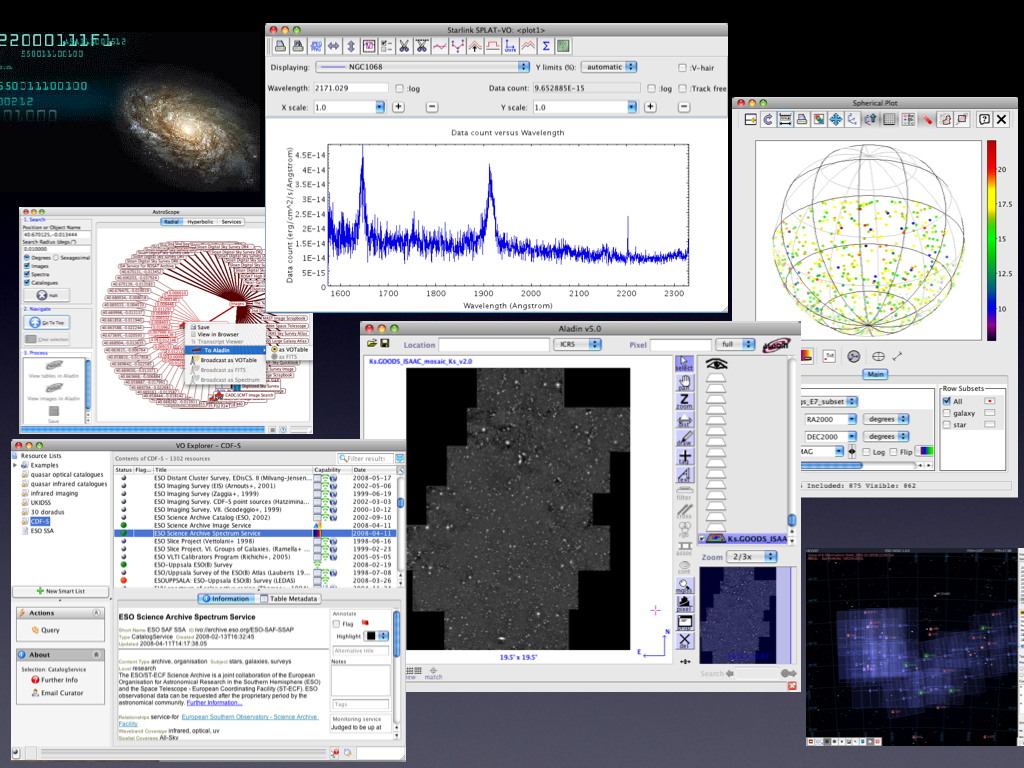
\includegraphics[width=\linewidth]{../images/votoolsworkshop.png}
\caption{Náhled pracovní plochy s nástroji VO}
\end{figure}

    Představte si, že chcete získat pozorování vámi zkoumaného objektu z
různých, ideálně všech dostupných, zdrojů. Jenže každá observatoř
používá jiné technické vybavení i konvence týkající se struktůry uložení
dat. Proto vznikla \textbf{I}nternational \textbf{V}irtual
\textbf{O}bservatory \textbf{A}lliance
\href{http://www.ivoa.net/}{IVOA}, která zaštiťuje její další rozvoj,
stejně jako World Wide Web Consortium (W3C) nepřímo definuje jakým
směrem se ubírá vývoj samotného Internetu, na němž jsme, a nebojme si to
přiznat, všichni tak trochu závislí.

    Virtuální observatoř je tedy souhrn nástrojů a protokolů pro získávání a
manipulaci s astronomickými daty unifikovaným způsobem bez nutnosti
starat se o rozdílné implementace na úrovni jednotlivých observatoří,
respektive datových archívů. Skrze virtuální observatoř je tedy možné
získat informace o astronomických objektech z různorodých zdrojů. Můžete
se dotazovat na souřadnice objektů na obloze podle jeho identifikátoru,
či právě naopak, zjistit, které objekty se nacházejí v okolí daných
souřadnic, tedy provést tak zvaný \emph{cone search}. Pro daný objekt,
nebo skupinů objektů definovanou různými parametry, můžete získat právě
ty informace, které vás zajímají. Ať už samotné snímky z přehlídkových
katalogů, světelné křivky či spektra. V neposlední řadě stojí za zmínku,
že ve Virtuální observatoři můžete nalézt taky nepřeberné množství
teoretických numerických modelů hvězdného vývoje.

    K virtuální observatoři můžete přistupovat různými způsoby. Tím
nejintuitivnějším je asi přímý přístup skrze webový prohlížeč, tak jak
jste zvyklí z každodenního brouzdání po webu. Jen vás nesmí odradit
formulářový vzhled jednotlivých stránek s množstvím polí pro zadávání
omezujících parametrů pro vyhledávání. Další možností je použití
specializovaných programů pro dílčí úkony, které však spolu mohou
navzájem komunikovat a vzájemně si vyměňovat data. Ty se v rámci
Virtuální observatoře přenášejí ve standardizovaném formátu, který je
astronomům vlastní, tedy \textbf{F}lexible \textbf{I}mage
\textbf{T}ransport \textbf{S}ystem (FITS), nebo speciálním formátu
virtuální observatoře \emph{VOTable}. Oba formáty umožňují oddělit
takzvaná \emph{metadata}, což je abstraktní popis skutečných dat nesoucí
navíc informaci o fyzikálních jednotkách umožňující jejich přesnou
interpretaci.

    Poslední možností, které se budeme dále podrobněji věnovat, je přímý
přístup ke službám Virtuální observatoře skrze aplikační rozhraní (API)
programovacího jazyka Python. Respektive pomocí k tomuto účelů speciálně
určenému balíčku \texttt{astroquery}, který je nepostradatelným
pomocníkem již dobře známého balíku AstroPy.

    \section*{Vyhledávání souřadnic}\label{vyhleduxe1vuxe1nuxed-souux159adnic}

    Začněme jednoduchým příkladem nalezení souřadnic známého blazaru
\emph{S5 0716+714}, tedy objektu typy BL Lac. K tomuto účelu se nám bude
hodit modul s fyzikálními jednotkami, objekt pro souřadnice a nakonec
objekt pro dotazování se astronomické databáze Simbad.

    \begin{Verbatim}[commandchars=\\\{\}]
{\color{incolor}In [{\color{incolor}2}]:} \PY{k+kn}{from} \PY{n+nn}{astropy} \PY{k}{import} \PY{n}{units} \PY{k}{as} \PY{n}{u}
        \PY{k+kn}{from} \PY{n+nn}{astropy}\PY{n+nn}{.}\PY{n+nn}{coordinates} \PY{k}{import} \PY{n}{SkyCoord}
        \PY{k+kn}{from} \PY{n+nn}{astroquery}\PY{n+nn}{.}\PY{n+nn}{simbad} \PY{k}{import} \PY{n}{Simbad}
\end{Verbatim}

    \begin{Verbatim}[commandchars=\\\{\}]
{\color{incolor}In [{\color{incolor}3}]:} \PY{n}{bllac} \PY{o}{=} \PY{n}{SkyCoord}\PY{o}{.}\PY{n}{from\PYZus{}name}\PY{p}{(}\PY{l+s+s2}{\PYZdq{}}\PY{l+s+s2}{S5 0716+714}\PY{l+s+s2}{\PYZdq{}}\PY{p}{)}
        \PY{n}{bllac}
\end{Verbatim}

            \begin{Verbatim}[commandchars=\\\{\}]
{\color{outcolor}Out[{\color{outcolor}3}]:} <SkyCoord (ICRS): (ra, dec) in deg
            (110.47270192, 71.34343428)>
\end{Verbatim}
        
    Teď když známe přesné souřadnice objektu na obloze, můžeme na něj
namířit teleskop či družici, nebo si v přehledné tabulce vypsat objekty
v jeho okolí.

    \begin{Verbatim}[commandchars=\\\{\}]
{\color{incolor}In [{\color{incolor}4}]:} \PY{n}{table} \PY{o}{=} \PY{n}{Simbad}\PY{o}{.}\PY{n}{query\PYZus{}region}\PY{p}{(}\PY{n}{bllac}\PY{p}{,} \PY{n}{radius}\PY{o}{=}\PY{l+m+mi}{5}\PY{o}{*}\PY{n}{u}\PY{o}{.}\PY{n}{arcmin}\PY{p}{)}
        \PY{n}{table}\PY{o}{.}\PY{n}{pprint}
\end{Verbatim}

            \begin{Verbatim}[commandchars=\\\{\}]
{\color{outcolor}Out[{\color{outcolor}4}]:} <bound method Table.pprint of <Table masked=True length=23>
                MAIN\_ID               RA      {\ldots} COO\_WAVELENGTH     COO\_BIBCODE    
                                   "h:m:s"    {\ldots}                                   
                 object             str13     {\ldots}      str1             object      
        ----------------------- ------------- {\ldots} -------------- -------------------
         7C 071610.69+712601.00 07 21 53.4484 {\ldots}              R 2009A\&A{\ldots}493..317L
                  [BKB2006b] G3  07 21 56.852 {\ldots}                1998yCat.1252{\ldots}0M
                  [BKB2006b] G1  07 21 51.418 {\ldots}                1998yCat.1252{\ldots}0M
                  [BKB2006b] G2  07 21 42.111 {\ldots}                1998yCat.1252{\ldots}0M
        2MASS J07215435+7119208   07 21 54.35 {\ldots}              I 2003yCat.2246{\ldots}0C
        2MASS J07221260+7121146   07 22 12.61 {\ldots}              I 2003yCat.2246{\ldots}0C
        2MASS J07214124+7119117   07 21 41.25 {\ldots}              I 2003yCat.2246{\ldots}0C
                TYC 4368-1025-1  07 21 33.374 {\ldots}              O 2000A\&A{\ldots}355L..27H
        2MASS J07215232+7118176   07 21 52.32 {\ldots}              I 2003yCat.2246{\ldots}0C
                            {\ldots}           {\ldots} {\ldots}            {\ldots}                 {\ldots}
        2MASS J07211606+7119551   07 21 16.06 {\ldots}              I 2003yCat.2246{\ldots}0C
        2MASS J07221061+7117497   07 22 10.62 {\ldots}              I 2003yCat.2246{\ldots}0C
        2MASS J07212077+7118480   07 21 20.78 {\ldots}              I 2003yCat.2246{\ldots}0C
        2MASS J07221803+7123344   07 22 18.03 {\ldots}              I 2003yCat.2246{\ldots}0C
        2MASS J07222820+7117374   07 22 28.20 {\ldots}              I 2003yCat.2246{\ldots}0C
                    [NMR2005] c   07 22 36.39 {\ldots}                2005AJ{\ldots}130.1466N
                 TYC 4368-870-1 07 22 36.4392 {\ldots}                1998A\&A{\ldots}335L..65H
        2MASS J07223155+7117499   07 22 31.56 {\ldots}              I 2003yCat.2246{\ldots}0C
          1RXS J072247.8+711821  07 22 47.801 {\ldots}                                   
        2MASS J07213751+7115518   07 21 37.51 {\ldots}              I 2003yCat.2246{\ldots}0C>
\end{Verbatim}
        
    Co s touto tabulkou dál dělat ponechávám již jen na fantazii zvídavého
čtenáře. Jako praktické cvičení si můžete například vykreslit polohy
nalezených hvězd. Taková mapka s okolím se vám může hodit, když se
rozhodnete pozorovat změny jeho jasnosti pro pořízení světelné křivky a
následnou konstrukci fázového portrétu odrážející jeho chaotické
chování.

    \section*{Atomické čáry}\label{atomickuxe9-ux10duxe1ry}

    Astrofyzikálně zajímavou aplikací využití Virtuální observatoře může být
i získání seznamu atomárních čar daného prvku v zadaném rozsahu vlnových
délek. Užitečnost této možnosti při studiu hvězdných spekter je snad
zřejmá.

    \begin{Verbatim}[commandchars=\\\{\}]
{\color{incolor}In [{\color{incolor}5}]:} \PY{k+kn}{from} \PY{n+nn}{astroquery}\PY{n+nn}{.}\PY{n+nn}{atomic} \PY{k}{import} \PY{n}{AtomicLineList}
\end{Verbatim}

    \begin{Verbatim}[commandchars=\\\{\}]
{\color{incolor}In [{\color{incolor}6}]:} \PY{n}{AtomicLineList}\PY{o}{.}\PY{n}{query\PYZus{}object}\PY{p}{(}\PY{n}{wavelength\PYZus{}range}\PY{o}{=}\PY{p}{(}\PY{l+m+mi}{400}\PY{o}{*}\PY{n}{u}\PY{o}{.}\PY{n}{nm}\PY{p}{,} \PY{l+m+mi}{600}\PY{o}{*}\PY{n}{u}\PY{o}{.}\PY{n}{nm}\PY{p}{)}\PY{p}{,}
                                    \PY{n}{element\PYZus{}spectrum}\PY{o}{=}\PY{l+s+s2}{\PYZdq{}}\PY{l+s+s2}{H}\PY{l+s+s2}{\PYZdq{}}\PY{p}{)}
\end{Verbatim}

            \begin{Verbatim}[commandchars=\\\{\}]
{\color{outcolor}Out[{\color{outcolor}6}]:} <Table length=3>
        LAMBDA VAC ANG SPECTRUM  TT  TERM J J    LEVEL ENERGY  CM 1  
           float64       str3   str2 str3 str3         str22         
        -------------- -------- ---- ---- ---- ----------------------
              4102.892      H I   E1  2-6  *-* 82259.11 -   106632.17
              4341.684      H I   E1  2-5  *-* 82259.11 -   105291.66
              4862.683      H I   E1  2-4  *-* 82259.11 -   102823.90
\end{Verbatim}
        
    Komplexní příklad demonstrující širší možnosti využití Virtuální
observatoře bude prezentován na praktickém cvičení. Nedočkavý jedinec se
může opět ponořit do samostudia dokumentace, plné názorných úkázek, obou
použitých balíčků.

\begin{itemize}
\tightlist
\item
  \href{http://docs.astropy.org/en/stable/}{AstroPy}
\item
  \href{http://astroquery.readthedocs.org/en/latest/}{AstroQuery}
\end{itemize}


    % Add a bibliography block to the postdoc
    
    
    
    \end{document}
